\section{Bildverarbeitung}\label{sec:linien}

Als haupts\"achliche Quelle f\"ur die Erfassung und Verarbeitung der Umwelt des Fahrzeugs haben wir das Bild
einer Webcam verwendet. Eine Kinect-Kamera mit Tiefenbild war zwar bereits auf dem Fahrzeug vorinstalliert,
jedoch beschlossen wir aus folgenden Gr\"unden, eine eigene Kamera zu verwenden:
\begin{itemize}
	\item Der flache Blickwinkel der Kinect erlaubte es nicht, den Boden unmittelbar vor dem Fahrzeug
	zu sehen. Die von uns verwendete Webcam dagegen konnte frei angebracht und der Blickwinkel
	(insbesondere dessen Steilheit) nach Belieben variiert werden.
	\item Die OpenCV-Bibliothek bot uns die M\"oglichkeit, den Webcam-Stream direkt einzulesen und
	daran Voreinstellungen vorzunehmen. Bei der Kinect w\"are hingegen eine Vorkonvertierung n\"otig
	geworden.
	\item F\"ur die von uns zu realisierenden Aufgaben (Fahrbahn- und Schildererkennung) war die
	zus\"atzliche Tiefenbild-Funktionalit\"at der Kinect wenig bis nicht relevant.
\end{itemize}

\begin{figure}[h]
	\centering
	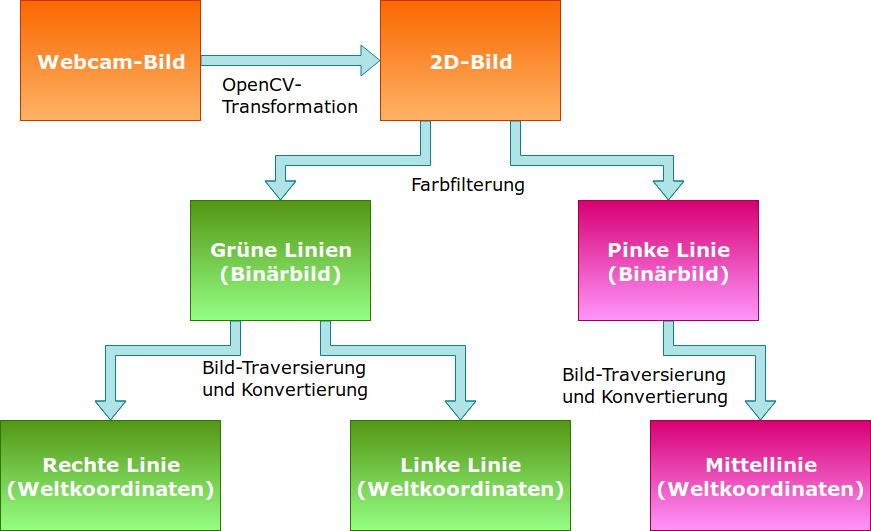
\includegraphics[width = 1.0\textwidth]{images/Bildverarbeitung.png}
	\caption{\"Ubersicht der einzelnen Schritte zur Bildverarbeitung}
	\label{fig:bildverarbeitung}
\end{figure}

Die groben Schritte, die f\"ur die Bildverarbeitung durchgef\"uhrt werden, sind in \figurename\ \ref{fig:bildverarbeitung} schematisch dargestellt.\\
Das eingelesene Webcam-Bild wird mithilfe der Bildverarbeitungs-Library OpenCV so transformiert, dass
der neue Bildausschnitt einer Draufsicht auf die Strecke aus der Vogelperspektive entspricht.
Davon ausgehend wird eine Farbfilterung vorgenommen, um die gr\"unen (Au\ss en-)Linien und die
pinke (innere) Linie jeweils in einem eigenen Bin\"arbild zu isolieren. Das Ergebnis wird
schlie\ss lich genutzt, um die Fahrzeugkoordinaten der einzelnen Linien zu bestimmen.\\
Die genauen Ma\ss nahmen, die f\"ur die Implementierung der einzelnen Verarbeitungsschritte getroffen 
wurden, werden im folgenden Abschnitt genauer vorgestellt.


\subsection{Kalibrierung der Kamera}

Beim Anbringen der Webcam wurde ein Blickwinkel gew\"ahlt, der zum einen eine m\"oglichst gute Sicht auf die
Strecke unmittelbar vor dem Fahrzeug erm\"oglicht, aber gleichzeitig ausreichend viel Strecke nach
vorne erfasst (auch um Verkehrsschilder noch gut erkennen zu k\"onnen).\\
Um eine korrekte Transformation des aufgenommenen Bildes in die Vogelperspektive erzielen zu
k\"onnen, musste eine Kalibrierung f\"ur die eingestellte Kamera-Position vorgenommen werden.

Zu diesem Zweck wurde ein Referenz-Rechteck aus Papier angefertigt und dessen reale Ma\ss e ausgemessen.
F\"ur die Kalibrierung wurde es im zentralen Sichtfeld der Kamera platziert, zus\"atzlich wurde der
Abstand zum Fahrzeug bestimmt.

- zwei Bilder nebeneinander: Foto des Rechtecks + Darstellung der Ma\ss e (technische Zeichnung)\\
- Beschreibung der ausgemessenen Dimensionen\\
- Testrechteck\\
- Klasse CameraCalibration + deren Funktionen\\
- Objekt der Klasse CameraCalibration entspricht immer einer bestimmten festen Kalibrierung und kann
an mehreren Stellen im Code wiederverwendet werden\\


\subsubsection{Umrechnung von Koordinaten}

- wie werden Ma\ss e f\"ur die Umrechnung verwendet?\\
- Methoden der Klasse CameraCalibration\\
- Umrechnung der Koordinatensysteme ineinander, Formeln\\

\subsection{Einlesen des Kamera-Bilds}

- Kamera-Aufnahme-Setup \"uber OpenCV (und rqt\_reconfigure)\\
- Beschreibung der Node (webcam\_publisher) / des Wrappers(CameraReader)\\

\subsection{Weiterverarbeitung des Kamera-Bilds}

- ImageProcessor erkl\"aren: bietet verschiedene Bildverarbeitungsfunktionen, enth\"alt Mat-Objekt\\
- Output: Bin\"arbild\\

\subsection{Detektion der Fahrbahnlinien}

- LanePointsCalculator: Funktionen zur Ermittlung bestimmter Punkte im Bin\"arbild\\
- LaneDetector: abstrakte Oberklasse für unterschiedliche Ans\"atze zur Erkennung von Fahrbahnmarkierungen\\
- TransformingLaneDetector: verwendete Klasse, welche die Hauptlogik enth\"alt\\
- Node lane\_detection: verwendet TransformingLaneDetector, Publishen + Subscriben\\


\textbf{TODO}\\
- eigene section für Monitoring-Funktionen + Debugging-Nodes\\